Confrontare i codici degli esercizi 14-17 per approssimare la funzione $f(x)=sin(x)$ sulle ascisse $x_\mathrm{i}=i\pi/n,i=0,1,...,n$, per $n=1,2,...,10$.
Graficare l'errore massimo di approssimazione verso $n$ (in semilogy), calcolato su una griglia uniforme di 10001 punti nell'intervallo $[0,\pi]$.

\hspace*{\fill}
\par\noindent\rule{\textwidth}{0.4pt}
\hspace*{\fill}

\begin{lstlisting}[language=Matlab, caption=Codice Matlab]
f = @(x) sin(x);
f1 = @(x) cos(x);
x = linspace(0, pi, 10001)';
fx = f(x);

el = zeros(10, 1); en = zeros(10, 1); eh = zeros(10, 1);
esn = zeros(10, 1); esnak = zeros(10, 1);
for n = 1 : 10
	xi = zeros(n + 1, 1);
	for i = 0 : n, xi(i + 1) = (i * pi) / n; end
	fi = f(xi);
	f1i = f1(xi);

	yl = lagrange(xi, fi, x);
	el(n) = norm(fx - yl, inf);

	yn = newton(xi, fi, x);
	en(n) = norm(fx - yn, inf);

	yh = hermite(xi, fi, f1i, x);
	eh(n) = norm(fx - yh, inf);

	if n >= 2
		ysn = spline3(xi, fi, x);
		esn(n) = norm(fx - ysn, inf);
	end

	if n >= 3
		ysnak = spline3nak(xi, fi, x);
		esnak(n) = norm(fx - ysnak, inf);
	end

end
x = 1 : 10;
semilogy(x, el, x, en, x, eh, x, esn, x, esnak);
legend('Lagrange', 'Newton', 'Hermite', 'Spline cubica naturale', 'Spline cubica not-a-knot');
\end{lstlisting}

La seguente figura mostra gli errori assoluti massimi dei vari metodi di interpolazione implementati:
\begin{figure}[H]
     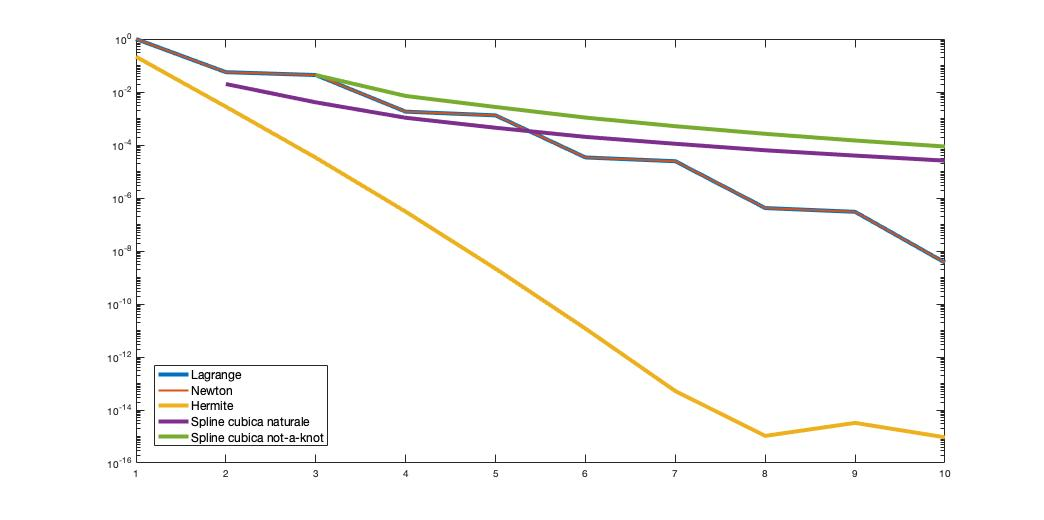
\includegraphics[width=\textwidth]{Chapter-4/Exercise-18/plot.jpg}
     \caption*{Errori assoluti commessi per approssimare la funzione con $n = 1: 10$}
\end{figure}
Si nota che, contrariamente a quanto accade usualmente con l'utilizzo di ascisse equidistanti, l'errore va a diminuire all'aumentare del numero di nodi di interpolazione. Questo risultato è dato dal fatto che la funzione in esame è molto regolare, ovvero appartiene alla classe $\mathbb{C}^{\infty}$.
